
\section{Introduction}
In classes at many universities professors have in-class graded quizzes and take attendance through the use of an Audience Response System (ARS). Students are required to purchase electronic answering devices commonly referred to as clickers.  As the professor displays a question for the class each student answers and the results typically are shown in an aggregated format to assess how the class did on each question.  This answering system is very useful because teachers and students can get real time feedback on how the class is learning the material.  At the University of Utah the Turning Point system provided by Turning Technologies is used.

ARSs are becoming very popular not just in schools but in other social gatherings.  Opinions and decisions of participants at political gatherings, game shows, and large committees all need a way to be gathered quickly and anonymously.  Delegates in the Republican Caucus in Utah, for example, use RF ARS
devices from Turning Technologies for voting on political candidates
and procedures.

When a RF ARS system is used, the base station will listen to a preset radio frequency. The clicker sends its unique Media Access Controller (MAC) address with an answer and an error-detecting code to prevent environment interference from mangling the response transmitted.  The clicker will transmit repeatedly until a response is detected from the base station.  The base station stores only the last received answer from each clicker so that responses from a clicker can change while the question is still open.

However this transmission is sent without any encryption.  Nor is there verification that the answer sent was transmitted from the clicker that uses the indicated MAC.  This means that by default the clicker traffic is open for attack by impersonation.  In this paper the authors constructed a device that sniffs and impersonates the radio traffic of the ARS used at the University of Utah but this device could also be used at the Republican Caucus.  This paper demonstrates how the current ARS in use, is vulnerable and how easy it would be for individuals to take advantage of the open traffic.  The paper will then make suggestions for securing the clicker.

\section{Related Work}

Back in July of 2010, Travis Goodspeed~\cite{travis} reverse engineered a Turning Point ResponseCard RF clicker which uses a NRF24E1 chip.  He demonstrated that sniffing packets from the clicker was possible and outlined his results.  As a conclusion to his results, he suggested attaching separate hardware to create a virtual student that could automatically vote with the majority for each quiz in class.

Two years later, Taylor Killian~\cite{taylor} took Goodspeed’s work and built a clicker emulator.  The emulator used an Arduino processor board for control and a NRF24L01 board to transmit and receive over the RF band. He implemented multiple features that could be used in the classroom including: sniffing packets, generating statistics, blocking audience responses, responding as a single clicker, responding as all clickers.  When sending answers to the base station the emulator could either send a selected answer for the MACs or a random answer.  Another useful feature was to auto-respond with the most popular answer used in class.

For this paper Killian’s work was expounded upon. The authors found that some of the emulator’s features were lacking in flexibility for testing in a classroom.  Also Killian's code worked well for ResponseCard RF models but not the NXT models now in production. The Arduino code was augmented with the ability to scan for channels in use, and the ability to specify which MACs to respond with.  Also the code was updated to allow the emulator to work with newer versions of the RF clickers.

In conjunction with the added features in the emulator, a Graphical User Interface (GUI) was created to more easily control the emulator. This allows the authors to dynamically aggregate audience MAC addresses and immediately use them to respond to questions (as opposed to hard coding the MAC addresses in the Arduino emulator).  Also the GUI allows for fine grain selection of MAC addresses to respond with.  It also allowed the user to define different subsets of random answers instead of a set range.


\section{Threat Model}
ARSs are becoming more widely adopted and are currently used to elect politicians, grade students, and make policy decisions based on group feedback.  ARSs use a base station that listens for radio frequency transmissions sent to a pre-configured address.  The ARS used at the University of Utah has all base stations listen for the address 0x123456 to receive answers.  Each transmission is sent without encryption so it is possible to sniff MAC addresses and answers belonging to students in a classroom.  Another attack path is that each base station only logs the last submitted answer from each clicker.  The authors don't test the Triton system provided by Turning Technologies because the system does employ encryption.

Any student can easily assemble and control a sniffing device from off-the-shelf components purchased on the Internet.  If the student wants to cheat he or she can program the device to gather statistics on answers provided by other students and respond to the base station with the highest chosen answer.  If the quizzes are graded on a curve it would provide incentive to change the answers of fellow students so that they miss the question.

At a political rally an individual might want to force a particular candidate to win or lose.  Legislation is directly influenced by who is voted into office. Another option is to jam a base station to cause a delay in decision making.  If an attack disrupts an ARS system enough then it will probably be replaced with another, costing the organization time and money in the process.

\section{Hardware}
The transmitter for the prototype was chosen based on what is currently in use by the clickers at school, the NRF24L01 wireless module.  The NRF24L01, see Figure~\ref{img:wirelessAdapter}, is an adapter that handles transmitting and receiving over the RF 2.4 GHz band.  It can be configured by setting registers based on commands from an external controller.

\begin{figure}[h]
\centering
  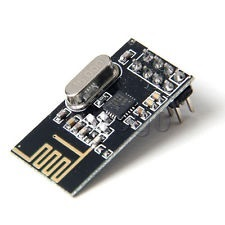
\includegraphics[scale=.6]{images/wirelessAdapter}
    \caption{NRF24L01 wireless module board~\cite{wirelessAdapterPhoto}}
	\label{img:wirelessAdapter}
\end{figure}

\begin{figure}[h]
\centering
  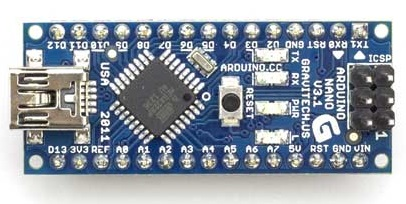
\includegraphics[scale=.6]{images/arduinoNano}
    \caption{Arduino Nano component board~\cite{ArduinoNanoPhoto}}
	\label{img:arduinoNano}
\end{figure}

\begin{figure}[h]
\centering
  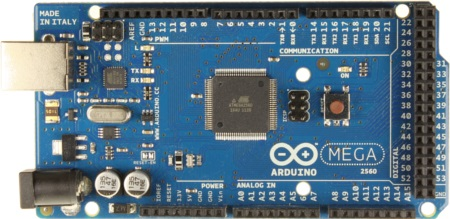
\includegraphics[scale=.6]{images/arduinoMega}
    \caption{Arduino Mega component board~\cite{ArduinoMegaPhoto}}
	\label{img:arduinoMega}
\end{figure}

 \begin{table}[b!]
\centering
	\begin{tabular}{|c|c|}
	\hline
\multicolumn{2}{|c|}{Arduino Nano} \\ \hline
Arduino Pins & transmitter Pins \\ \hline
D8 & IRQ \\ \hline
D9 & CE \\ \hline
D10 & CSN \\ \hline
D11 & MOSI \\ \hline
D12 & MISO \\ \hline
D13 & SCK \\ \hline
\multicolumn{2}{c}{} \\ \hline
\multicolumn{2}{|c|}{Arduino Mega} \\ \hline
Arduino Pins & transmitter Pins \\ \hline
41 & IRQ \\ \hline
42 & CE \\ \hline
50 & CSN \\ \hline
51 & MOSI \\ \hline
52 & MISO \\ \hline
53 & SCK \\ \hline
\end{tabular}
        \caption{Pinouts for connecting NRF24L01 wireless adapter board to Arduino controllers}
	\label{table:pinouts}
\end{table}

The two controllers chosen for experimenting were an Arduino Nano, see Figure~\ref{img:arduinoNano}, and an Arduino Mega, see Figure~\ref{img:arduinoMega}.  Both Arduino boards connected to a laptop using a USB cable.  Communication with the Arduinos was handled though a virtual Communication Port (COM) driver. 

To connect the Arduino processor boards to the wireless module the pinouts in Table~\ref{table:pinouts} were followed.  

Together the cost of hardware was \$3 for the NRF24L01 board and about \$10 for the Arduino Nano board.  This total price of \$13 is far cheaper than purchasing a clicker from the vendor which usually cost about \$40.  This might be incentive enough for students to construct their own device.

\section{Software}
To make the prototype easier to test and control, a GUI was programmed in C\#, see Figure~\ref{img:GUI}.  The GUI allows the user to do everything that was previously implemented by Taylor Killian.  However it also extended the capabilities of the emulator. The code communicates to the arduino board through the Serial COM Port Libraries built into C\#. A laptop is connected to the arduino with a USB-to-serial adapter and in the software the user enters which COM number is used by the device. The channel used by the base station in a class room will also need to be entered before the Clicker Tricker can detect any transmitted packets.

\begin{figure*}[t!]
\centering
  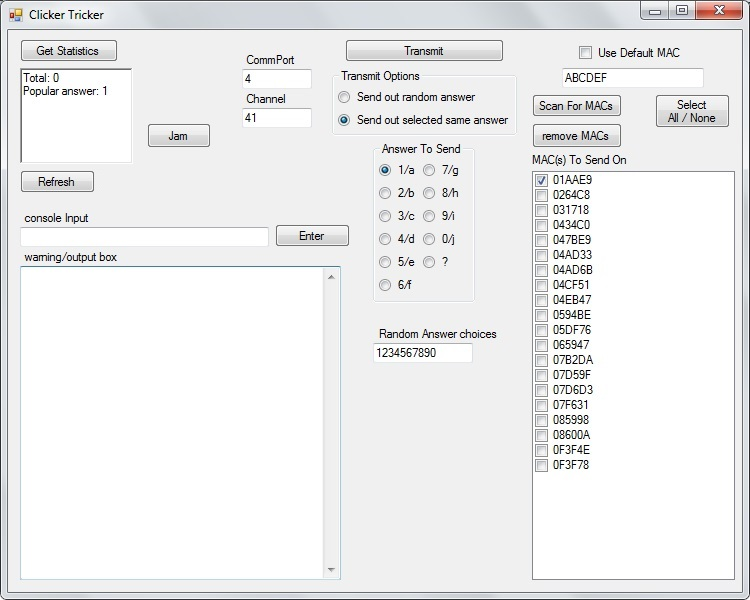
\includegraphics[scale=.8]{images/UI_ClickerTricker}
    \caption{GUI for controlling and testing the Clicker Tricker}
	\label{img:GUI}
\end{figure*}

The MAC list starts empty but after clickers start transmitting to the base station the MAC addresses and answers are stored on the Arduino.  The user only has to click a button to get a list of all available MACs or statistics of what is the most popular answer at the moment.  The UI was also programmed with a console interface to the Arduino controller board so that users can directly control it.
%After the MACs are collected the UI allows selective answering from the list.  This means that while a user might collect the answers for all students in the class he or she can answer for a subset of the students without worry of changing everyone's answer.

Once a list of MACs has been intercepted, the user has several options:
\begin{itemize}
\item Select all or a subset of the MACs to transmit with.
\item Jam all subsequent transmissions to a base station by sending a constant carrier signal.
\item Choose to respond as all selected MACs with the same answer.
\item Choose to respond with a random answer for each selected MAC.
\item See the answering statistics for all detected MACs, this would allow the user to see what is the most popular answer.
\end{itemize}

The UI was designed to allow full functionality of the Clicker Tricker.  It would be very easy to port the GUI to another coding language.  The authors feel that a smart phone could easily be programmed to control the Clicker Tricker.  This would alleviate the need of a laptop making it even harder to detect someone using the Clicker Tricker to cheat or cause disruption with an ARS.

\section{Tests and Results}

\subsection*{Experiment One}

Upon creating the working prototype above, permission was received from Professor James de St. Germain, refereed to as Jim, to use his CS3500 class to test the Clicker Tricker.  Jim had 142 students in his class. Twenty students had previously installed an app for their smart phones that interfaced with the base station through the professor's laptop by means of the WiFi network at the school.  The cell phone responses couldn't be picked up or modified by the Clicker Tricker but they could be disrupted as is shown in the jamming test.

For this set of experiments four phases were determined for testing:
\begin{enumerate}
\item Have students respond to a question so that MAC addresses and statistics could be gathered.
\item Have all students respond with the same answer and use the Clicker Tricker to change the answers to another option.
\item Have all students respond with the same answer and use the Clicker Tricker to change each of the answers to a random answer.
\item Stop students from answering by jamming the receiver.
\end{enumerate}

\textbf{Test 1 Results:}\\
Approximately 52 clickers were intercepted during the first experiment.  There were several different types of clickers being used in the class and several had different answer sets. Some had the option to answer with a number between 0-9 while others had the option to answer with a letter between a-j.  Some clickers even responded uppercase letters A-J. 



\textbf{Test 2 Results:}\\
When the professor posted the question for the second phase, the Clicker Tricker was used to try to change all the students responses from A to B, however when the results were shown it could be seen that none of the responses had been changed.

\textbf{Test 3 Results:}\\
The third phase was used to test the randomize responses functionality and the Clicker Tricker did send random answers but the results didn't show up in the results to the students.

\textbf{Test 4 Results:}\\
For phase 4 the clicker tricker was programmed to send out a constant carrier signal.  The signal was designed to stop the base station from detecting the student's responses to the posted question.  The clicker tricker was able to jam the signal of any clicker used by a student.  Some of the students using the phone application were still able to submit a response to the question.  However since the base station's resources were mainly utilized by the clicker tricker, not all of the students using phone applications were able to respond correctly.

\textbf{Conclusions from Experiment One:}\\ 
It looked like the Clicker Tricker failed, however for each question that the Clicker Tricker responded Jim had more than 130 extra student responses.  After the class, the results stored in the ARS software revealed that the Clicker Tricker had been responding to each question but instead of using the MACs collected it had transmitted on MACs hard coded into the Arduino processor code.

Another problem discovered is when a letter was transmitted as the answer. The arduino, due to the processor code, recorded a letter answer with an offset of one. For example, if the user sent out a/A the Arduino received b/B so when statistics were generated all of these different answer sets were displayed in the collected statistics.  Due to this offset the Clicker Tricker couldn't reliably report on the most popular answer or transmit the intended answer.  For example, If B was sent, A was received by the base station. If C was sent then B was received by the base station. 

After reviewing the results of the first experiment and borrowing Jim's base station, the Arduino code was fixed so that correct responses were sent and received.  Also the hard coded MAC addresses were removed so that the Clicker Tricker would only transmit collected addresses from the students in the class.

\subsection*{Experiment Two}

After fixing the Arduino processor code and forcing the UI to only answer with numbers, the Clicker Tricker was tested again in Jim's Class. Jamming wasn't retested as it had worked correctly the first time.  Impersonation of students was selected for this round of testing, so the following phases were selected:
 \begin{enumerate}
\item Have students respond to a question so that MAC addresses and statistics could be gathered.
\item Have all students respond with the same answer and use the Clicker Tricker to change the answers to another option.
\item Have all students respond with the same answer and use the Clicker Tricker to change each of the answers to a random answer.
\item Wait until students leave and answer using the collected MAC addresses.
\end{enumerate}

\begin{figure}[h!]
\centering
  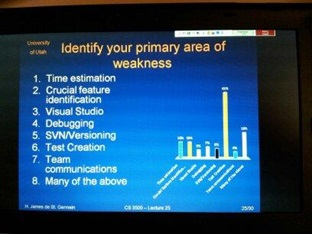
\includegraphics[scale=.95]{images/ARSStatistics}
    \caption{ARS reported, student answers for Test 1 question.}
	\label{img:ARSStatistics}
\end{figure}

\begin{figure}[h!]
\centering
  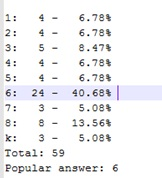
\includegraphics[scale=1]{images/TrickerStatistics}
    \caption{Clicker Tricker results sniffed from student's clickers for Test 1 question.}
	\label{img:TrickerStatistics}
\end{figure}

\textbf{Test 1 Results:}\\
This time 59 clickers were picked up during the first two questions, later seven more were detected after moving the clicker tricker to a different part of the room.  The ARS software used by the base station aggregated the results from class and Figure~\ref{img:ARSStatistics} is the result.  The ARS software displayed the most popular answer to be number six followed by number eight. Figure~\ref{img:TrickerStatistics} shows the output of the statistics from the Clicker Tricker.  Even though only about 45 percent of total responses were intercepted the Clicker Tricker was still able to determine the most popular answer.

\textbf{Test 2 Results:}\\
Once the students had left the class the questions were reposted and the Clicker Tricker was used to impersonate them. It was able to send a specific answer for each MAC address that had been intercepted and all the answers sent were received by the receiver.

\textbf{Test 3 Results:}\\
Sending random answers for each of the 66 clicker addresses that had been intercepted was also successful and the distribution of answers was fairly random. The receiver did get every single answer sent and things were working the way they were supposed to be.

\textbf{Conclusions From Experiment Two:}\\
The results from the second experiment showed that the Clicker Tricker was capable of sniffing student's traffic in real-time.  From about half of the clickers in the room the MAC addresses and answers were collected.  For each collected MAC address the Clicker Tricker was able to successfully impersonate the student by changing the base station's recorded answer after the student had responded.

The Clicker Tricker was tested with three different versions of clickers in use by students on campus.  However, it's possible that incompatible versions were present in the class which would explain why the Clicker Tricker couldn't detect all clickers in use by students.  Further investigation will need to be done to determine why only half the clickers in class were successfully sniffed.

\section{Suggestions for securing the clickers}
As they are now, the RF clickers in use at the school have no security measures to prevent sniffing of traffic or impersonation of users.  The same version of clickers that were detected in the experiments are in use in the Republican Caucus of Utah. All responses from the clickers are sent over the RF band and there is no encryption to safeguard the answers.  This means that an attacker could easily change the answers received by the base station by using the clicker's MAC address.  Because of this flaw the voting habits of the Caucus may be tampered with.  Students might cheat in class, or sabotage other students in their class.

To secure the clickers hardware and software changes could be implemented.  Because hardware is more costly to alter this paper will first propose software changes.  One solution to avoid the impersonation of a clicker would be to have the base station send a message after the response time period ends.  The message would contain the last answer received and the clicker would need to display this answer to the user.  Later versions of the clickers have an LED display so this seems like a plausible solution.  If the answer received on the clicker is different then what was sent then the user would be alerted to tampering.  After each student receives his or her answer the professor could then show the results for analysis.

Another solution would notify the user after each submission of an answer. When the user selects an answer to send, the clicker repeats many times its message to the base station until the station responds that the answer was received.  As part of the response it could include the previous answer received.  This solution would require the user or clicker to remember what was sent from a previous question.

The last software solution is to force the base station to alert the user each time an answer associated with their MAC address is changed.  After each answer is received the base station would send a message to the associated clicker based on MAC address.  The message would simply transmit what answer was just received.  The clicker would need to remember what was last sent and compare the two answers.  If the answers are different then it can alert the user that someone else has just submitted an answer for them.

These previous suggestions only stop impersonation but don't prevent eavesdropping to stop students from cheating.  Encryption of the transmissions would be the best solution for fixing the clickers.  The whole transmission would need to be encrypted with some padding bytes to foil attempts at decryption by an attacker.   This solution might require a hardware change as it would probably need more processing power or storage space on the clickers to handle the encryption and decryption algorithms.  This solution would probably raise the price of the clicker as well.  At the moment, Turning Technologies does manufacture a RF clicker that uses encryption, however the University hasn't implemented it for normal classroom use.

None of these suggestions will stop an attacker from jamming the system however.  The authors suggest at least one of these solutions be headed so that clicker traffic can be made safer.

%  used in many classes at the University of Utah and for voting in the Republican Caucus have no security measures to prevent eavesdroppers from listening in on answers being sent and the address of the responding clicker. They also have no security measures to prevent active attackers from changing answers or using collected data for their own purposes. All answers are sent in the clear on the RF band and, as mentioned above, the messages sent from the clicker to a receiver consist of 4 bytes. The first 3 bytes hold the clicker's MAC address and the last byte holds the user's answer.

%The responses from these clickers can be listened in on quite easily and if they are going to be used for voting in the Republican Caucus or to measure participation in classes at the University they should have some type of security measures to protect the users from passive and active attackers. Ideally the security to be added would not require changes to the hardware as that’d be fairly expensive for the creators and users would not be happy to have to pay for a new clicker that would likely be more expensive for them as well. 

%There are several options that could be implemented but would require follow up from the users if suspicious behavior is seen. One option could be, depending on the type of clicker and if it had an LCD screen, once a question is closed and before the results are displayed, the receiver could send a response to each clicker that participated in the poll and let it know what the last answer it received from that clicker was. The last answer for each participating clicker is all the receiver saves and it should always be the answer the user pressed. If the user notices the answer is different they should notify someone and the person trying to modify the users answers would be detected. This would not prevent anyone from listening in on answers and using the collected data for their own purposes. It would be a security measure that would need to be enforced by users and would be fairly trivial for the manufacturers to implement in the software. No hardware modifications should be needed to add this functionality to the clickers.

%Another similar option that could be implemented is to have the receiver take note every time it receives an answer for a particular MAC and immediately respond with that answer notifying the clicker that it has received an answer from the clicker’s MAC address and showing the user what that answer was. If an active attacker were present and was sending out new answers for the MAC addresses they’d intercepted, the user would receive the base station’s response every time the attacker tried changing their answer. Again if suspicious behavior were detected by the user they should let the coordinator know immediately. 

%The last option like this would be to simply send the answer recorded for the previous question every time a new question is answered. The receiver is already sending out a response to the clickers to let them know their answer was received, it could include the previous question’s response and the user can verify it is accurate. Displaying the previous answer on the LCD screen should be trivial for the manufacturers and can help users to know their answers are not being changed. 

%There are other security measures that could be added as well, but to implement them the hardware in the clickers would likely need to be modified. To prevent eavesdroppers from listening in on responses and the answers that are sent for each MAC address, the clicker and the receiver can perform an initial handshake to establish a secret key between the two that can be used to encrypt answers sent from the clickers and responses sent from the receiver. Once the secret key is established it should be used to encrypt the data being sent out as well as several bytes of padding. Since the clicker’s are only sending out four bytes when answering a question there wouldn’t be a lot of potential variety in the encrypted output and it would be easier for an attacker to break. Adding additional bytes of padding increases the size of the encrypted data requiring an active attacker to perform more work.

%Whether it's adding security measures that would need to be enforced by the users or adding security measures that require a hardware change to the clickers, security is needed on these devices. Right now it is actually cheaper to buy the hardware to set up everything needed to intercept and send new answers for particular MAC addresses than it is to buy a clicker. They are being used to gather important information and, in the case of the Republican caucus, are being used to vote for candidates or potential procedures to put in place and in the classes at the University of Utah they’re frequently used to answer questions or keep track of the student’s participating in the class. The people using the clicker’s should be able to have their responses secured against attackers.


\section{Conclusion}

The test results show that the Clicker Tricker is an effective device for impersonating and jamming the clickers of fellow students.  While the Clicker Tricker didn't successfully collect the MACs of all students, it still collected the MACs of 44.3 percent of the class.  Even this amount of addresses can be used to cause problems.

With more work a solution could be found that could collect all the MACs from Jim's class.  If a majority of MACs are intercepted the person controlling the Clicker Tricker could potentially control the grading curve of each quiz in class.  Of bigger concern is the use of unencrypted clickers in a political environment because the results have a farther reaching effect than an individual's grades.
However, simple steps could be taken to prevent an unknown attacker from causing problems in a classroom.

It is apparent that security through obscurity is no longer an option for the RF clicker.  The code for controlling a clicker emulator is easily found on the Internet and with just \$13 anyone can make his or her own Clicker Tricker.


\begin{comment}
%\section{Methods for collecting data}

\begin{figure}[h]
\centering
  \includegraphics[scale=.5]{graphs/flowDiagram}
    \caption{Netflow Architecture~\cite{wiki.netflow}}
	\label{fig:flowdiagram}
\end{figure}

\begin{table}[h]
\centering
    \caption{minimum flow characteristics~\cite{wiki.netflow}}
	\begin{tabular}{|p{4.5cm}|}
	\hline
Ingress interface \\ \hline
Source IP address \\ \hline
Destination IP address \\ \hline
IP protocol\\ \hline
Source port if available \\ \hline
Destination port if available \\ \hline
IP type of service \\ \hline
\end{tabular}
	\label{table:commonFlowData}
\end{table}

Figure~\ref{fig:flowdiagram} in Table~\ref{table:commonFlowData}.  More data than these seven characteristics can be collected but these are the minimum. 

\end{comment}
